\documentclass[12pt]{article}

\usepackage[vmargin=25mm, hmargin=20mm]{geometry}
\usepackage{parskip}
\usepackage{graphicx}
\usepackage{minted}
\usepackage{booktabs}
\graphicspath{ {../figures/} }

\begin{document}
\title{Hash Table Performance}
\author{Ben Ellis}
\date{\today}
\maketitle

\section*{Introduction}
% Decided to implement chained (and possibly open addressed) hash table.
% Investigate effects of these choices on the read and write performance
In this report I present an investigation into different implementations of
a hash set which stores unsigned 32 bit integers. 

A hash set stores integers by using a hash function, $h$, to compute an index
into an array from the input and then storing the element in that location. 
In the case of two elements mapping to the same location, called a conflict, there are two main
courses of action. The first is to continue probing other indices in the array until
a free slot is found, and the second is to extend the array into an array of linked lists, and
attach the element at a free slot later in the table. This form of hash table is illustrated in
Figure~\ref{fig:chaining}.

% Explain how a chained and open-addressed hash table works
\begin{figure}
    \centering
    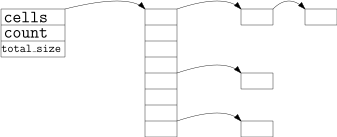
\includegraphics[width=0.5\textwidth]{chained_table}
    \caption{Diagram illustrating a chained hash table}\label{fig:chaining}
\end{figure}

\section*{Implementations}

I started by implementing a simple hash table with collision resolution via chaining. 
The definitions for the structs required are shown in Listing~\ref{fig:def}. Notice that
the table contains a pointer to a pointer to a value, that is there must be 2 memory 
references (and potentially two cache misses) before a value can be accessed. This is a
disadvantage compared to open addressing where the values are stored directly in the table.
\begin{listing}
    \centering
    \begin{minipage}[t]{.5\textwidth}
    \begin{minted}{C}
    typedef struct CELL {
        struct CELL *next;
        uint32_t val;
    } cell_t;
    typedef struct TABLE {
        uint32_t count;
        uint32_t total_size;
        cell_t **cells;
    } table_t;
    
    table_t *create_table();
    void insert(table_t *, const uint32_t);
    bool contains(table_t *, const uint32_t);
\end{minted}
\end{minipage}
\caption{Code for the initial definition of the chained hash table}
\label{fig:def}
\end{listing}

Inserting into the table is done by hashing the integer to find the index at which to insert it, and following the linked
list to the end before adding a new cell there. Checking a value is present in the table follows a similar process, but
checks for the presence of the value rather than inserting a new one. The only wrinkle is resizing the table. When the 
table reaches above a certain occupancy, it is doubled in size to retain performance. This is done by finding the 
correct index in the new table at which to insert the new value, and copying the cell to the end of the linked list.

I implemented a few simple tests to benchmark the performance of this data structure. The first inserted the integers
in the range $[0, 10^7)$ in order into the table, and then read them out in order. The results are shown in the 
Ordered Write and Ordered Read columns of Table~\ref{tab:perf} respectively. The second set of tests inserts some random
numbers into the table and reads either one of these numbers or a random number. The choice of whether to read a number 
that is in the table or one that is likely not is chosen at random. One test of this type inserts $256$ integers 
and reads $10^7$ times, and the other does the opposite, writing $10^7$ integers and reading $256$ times. These are 
listed in Table~\ref{tab:perf} as Random Read and Random Write respectively. 

\begin{table}
    \begin{tabular}{ccccc} \toprule
        Algorithm & Ordered Write (s) & Ordered Read (s) & Random Read (s) & Random Write (s) \\
        Chaining & $4.34 \pm 0.04$ & $\mathbf{0.34 \pm 0.03}$ & $1.94 \pm 0.02$ & $4.21 \pm 0.05$ \\
        Multi-element Chaining & $\mathbf{3.49 \pm 0.07}$ & $0.479 \pm 0.005$ & $\mathbf{1.88 \pm 0.03}$ & $\mathbf{3.43 \pm 0.02}$ \\
        \bottomrule
    \end{tabular}
    \caption{Results of benchmarking the different algorithms. Best results are in bold.}
    \label{tab:perf}
\end{table}

\end{document}
